\documentclass{beamer}

\usepackage{graphicx,hyperref,udesc,url}
\usepackage[utf8]{inputenc}
\usepackage[T1]{fontenc}
\usepackage{booktabs}
\usepackage[portuges]{babel}


\title[Métodos de Solução de PLI]{Análise de métodos para resolução de problemas de programação linear inteira}

\author[Renan S. Silva, Omir Alves]{
    Renan S. Silva, Omir Alves\\\medskip
    {\small \url{uber.renan@gmail.com}} \\
    {\small \url{@gmail.com}}
}

\institute[UDESC]{
    Departamento de Ci\^encia da Computa\c{c}\~ao \\
    Centro de Ci\^encias e Tecnol\'ogias\\
Universidade do Estado de Santa Catarina}

\begin{document}

\begin{frame}
    \titlepage

\end{frame}

\begin{frame}
    \frametitle{Sumário}
    \tableofcontents
\end{frame}

\section{Introdução}
\begin{frame}
    \frametitle{Introdução}

    Um problema a ser analisado e resolvido pode ser modelado com ferramentas matemáticas. Com o modelo
    matemático em mãos, pode-se resolver o problema original. Um dos meios de modelar problemas consiste na
    utilização da programação linear inteira (PLI).
\end{frame}

\begin{frame}{Introdução}
    \frametitle{Introdução}

    A um problema é dito de PLI se sua função objetivo e suas restrições são lineares e suas variáveis são inteiras.
    Caso algumas varáveis sejam reais, o problema é dito ser de programação linear inteira mista (PLIM). Para
    problemas na qual todas as variáveis deve ser $1$ ou $0$, diz-se que é um problema de programação linear inteira binária (PLIB).
\end{frame}

\begin{frame}{Modelagem}
    Um modelo geral de PLI é dado por:
    \begin{equation}
        max\{cx : Ax \leq b,x \geq 0, x \in \mathbb{Z}^{*} \}
    \end{equation}

    Onde $A \in \mathbb{R}^{m \times n}$, $c^T \in \mathbb{R}^n$, $x \in \mathbb{R}^n$ e $b \in \mathbb{R}^m$;
\end{frame}

\begin{frame}[c]{Exemplo}
    \frametitle{Problema do caminho mínimo}
    \begin{align}
        \text{z }&= \text{ min } \sum_{(i,j) \in A} c_{ij}x_{ij} \\
        \sum_{k \in V^+ (i)} x_{ik} - \sum_{k \in V^- (i)} x_{ki} &= 1,\text{ para } i = s \\
        \sum_{k \in V^+ (i)} x_{ik} - \sum_{k \in V^- (i)} x_{ki} &= 0,\text{ para } i \in V \backslash \{s, t\}  \\
        \sum_{k \in V^+ (i)} x_{ik} - \sum_{k \in V^- (i)} x_{ki} &= -1,\text{ para } i = t \\
        x_{ij} &\geq 0\text{ para } (i, j) \in A \\
        x \in Z^{\textbar A \textbar}
    \end{align}
\end{frame}

\section{Complexidade}
\begin{frame}[c]{Complexidade}
    A PLI e suas variantes são todas problemas NP-completos, de modo que o problema rapidamente torna-se
    intratável para instancias maiores. Em teoria da computação, a classe dos problemas NP-completos correspondem
    aos problemas que não podem ser resolvidos de modo eficiente (em tempo polinomial).
\end{frame}

\section{Métodos de solução}
\begin{frame}[c]{Métodos de solução}
    Foram considerados dois métodos de solução para este trabalho:
    \begin{itemize}
        \item \textit{branch and bound};
        \item \textit{branch and cut}.
    \end{itemize}
\end{frame}

\begin{frame}[c]{\textit{Branch and Bound}}
    O método de \textit{Branch and Bound} (BnB), consiste em dividir o espaço de busca $S$ em regiões menores $S_1, S_2, \ldots, S_n$, de modo
     que $S_1 \cup S_2 \cup \ldots \cup S_n = S$. Para cada subespaço é avaliado os seus limites inferiores e superiores, e com base
     nos limites é efetuada subsequente divisões até que um resultado suficientemente bom seja encontrado.
\end{frame}

\begin{frame}[c]{\textit{Branch and Cut}}
    O método de \textit{Branch and Cub} (BnC), funciona de modo semelhante ao BnB, no entanto utiliza-se planos de corte
    para melhorar os limites, fazendo com que menos nós(sub espaços) sejam explorados.

    Foram considerados 4 planos de cortes para este trabalho:
    \begin{itemize}
        \item Cortes de Gomory(GMI);
        \item Cortes por arredondamento inteiro misto(MIR);
        \item Cortes clique;
        \item Cortes de cobertura;
    \end{itemize}
\end{frame}

\begin{frame}[c]{Planos de Corte}
    Um plano de corte consiste em um hiperplano que remove uma área infactível do espaço de busca sem remover a solução ótima.
    Os planos de cortes são derivados algoritmicamente a partir das restrições do problema original, e cada plano de corte
    adiciona uma nova restrição ao problema. Portanto cada novo plano de conte introduzido ao problema o deixa
    mais difícil de resolver e reduz o espaço de busca.
\end{frame}

\section{Experimentos, resultados e análise}
\begin{frame}[c]{Experimentos}
    Utilizou-se as implementações do BnB e BnC com os cortes mencionados feita no solver GLPK. Resolveu-se todas
    as instâncias da MIPLIB com o solver e coletou-se diversas métricas de desempenho, tais como número de nós na
    arvore de enumeração, planos de cortes aplicados, gap, tempo e memória consumidos.
\end{frame}

\begin{frame}[c]{Resultados}
    \begin{table}[h!]
        \small
        \centering
        \begin{tabular}{l  l | l | l | l | l | l | l |} \cline{3-8}
            & \multicolumn{1}{l|}{} & \multicolumn{3}{c|}{\textit{Branch and Bound}} & \multicolumn{3}{c |}{\textit{Branch and Cut}} \\ \cline{2-8}
            \multicolumn{1}{l|}{}             & Tempo(s)              & Sucesso & Falha & Erro & Sucesso & Falha & Erro \\ \cline{1-8}
            \multicolumn{1}{|l|}{Cen\'ario 1} & 1800 s                & 35 & 30 & 5  & 45 & 20 & 11 \\ \hline
            \multicolumn{1}{|l|}{Cen\'ario 2} & 3600 s                & 39 & 26 & 6  & 48 & 17 & 11 \\ \hline
            \multicolumn{1}{|l|}{Cen\'ario 3} & 7200 s                & 43 & 22 & 6  & 52 & 13 & 11 \\ \hline
        \end{tabular}
        \caption{Resultados do \textit{Branch and Bound} e \textit{Branch and Cut}}
        \label{tabela_bnb_tempos}
    \end{table}

    Resultados observados:
    \begin{itemize}
        \item BnC resolveu mais instâncias que o BnB;
        \item A utilização de planos de corte introduziu diversos erros numéricos ao problema;
        \item BnC não conseguiu resolver algumas instâncias que o BnB consegue.
    \end{itemize}
\end{frame}

\begin{frame}[c]{Análise de algumas instancias}
    Observando o comportamento do solver pode-se identificar pontos relevantes ao desempenho de cada método.
    Analisou-se estas informações para entender o impacto do uso de planos de corte no processo de solução.
    Duas instâncias do MIPLIB são apresentadas a seguir:

    \begin{description}
        \item[air05] Instância que modela rotas de voo.
        \item[qiu] Instância que modela redes de fibras óticas;
    \end{description}
\end{frame}

\begin{frame}[c]{air05}
    \begin{figure}[htpb]
        \centering
        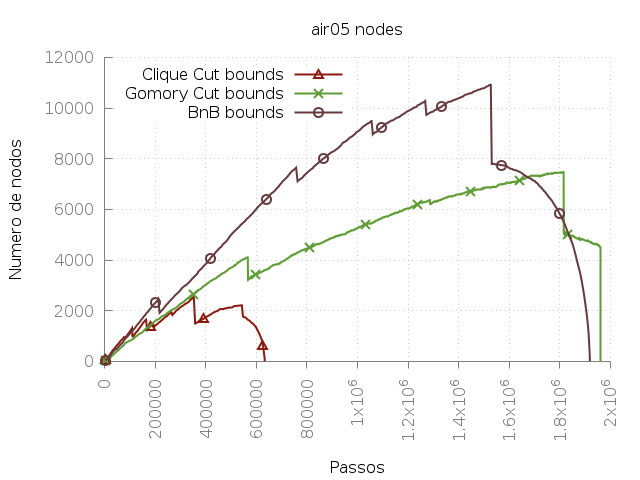
\includegraphics[width=0.8\linewidth]{air05_nodes}
        \caption{Número de nós}
    \end{figure}
\end{frame}

\begin{frame}[c]{qiu}
    \begin{figure}[htpb]
        \centering
        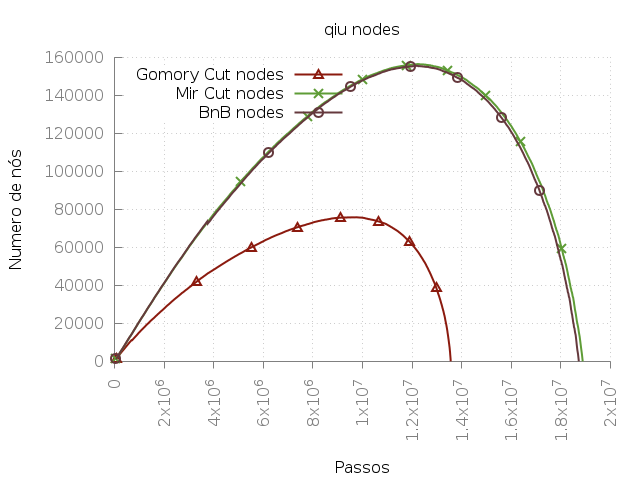
\includegraphics[width=0.8\linewidth]{qiu_nodes}
        \caption{Número de nós}
    \end{figure}
\end{frame}

\section{Considerações finais}
\begin{frame}[c]{Considerações Finais}
    Com este estudo pode-se identificar os principais métodos na literatura para a solução de problema de PLI. Observou-se
    o impacto da utilização de planos de corte no processo de solução. Pode-se ainda observar que:

    \begin{itemize}
        \item O BnC introduziu um número considerável de erros numéricos;
        \item O BnC em média obteve um desempenho superior ao BnB;
        \item O BnB foi capaz de resolver instâncias que o BnC não pode, devido as erros númericos
            ou aumento no tempo necessário para a computação;
    \end{itemize}
\end{frame}

\end{document}
